\begin{figure}[!h]
\centering
%\figuretitle{Figure~\ref{fig:filament_cavity}}
\begin{conditionalpanel}
    \begin{tikzcanvas}{}
    %
    \node(axialdimer)[inner sep=0pt,below right]{\includegraphics[width=\linewidth,height=1.25in,keepaspectratio]{../results/cavity/output/dimer_cavity_axial_cropped.png}};
    %
    \path (axialdimer.north)++(-0.25,-1.35) coordinate (axialdimerROISW1);           
    \path (axialdimer.north)++(0.25,-2.1) coordinate (axialdimerROINE1);
    \node(axialdimerROIrect) [fit={(axialdimerROISW1) (axialdimerROINE1)}, dashedrectanglefit] {};
    %
    \node(captionA)[inner sep=0pt,above left] at (axialdimer.north west) {\normalsize\textbf{\figurepanela}};
    %
    \path (axialdimer.south west)++(0.4,-0.5) coordinate (chainArotated);           
    \path (axialdimer.south east)++(-0.4,-0.5) coordinate (chainBrotated);
    %
    \node(chainArotatedlabel) [above, inner sep=2pt, align=center] at (chainArotated) {Chain A};
    \node(chainBrotatedlabel) [above, inner sep=2pt, align=center] at (chainBrotated) {Chain B};
    %
    %
    %
    \node(axialdimerapbs)[inner sep=0pt,right=0.5cm of axialdimer]{\includegraphics[width=\linewidth,height=1.25in,keepaspectratio]{../results/cavity/output/dimer_cavity_apbs_axial_no_ramp_cropped.png}};
    %
    \node(axialdimerlabel) [below, inner sep=2pt, align=center] at (axialdimerapbs.south) {Solvent-Exposed Side\\(Filament End Cap)};
    %
    \path (axialdimerapbs.north)++(-0.25,-1.35) coordinate (axialdimerapbsROISW1);   
    \path (axialdimerapbs.north)++(0.25,-2.1) coordinate (axialdimerapbsROINE1);
    \node(axialdimerapbsROIrect) [fit={(axialdimerapbsROISW1) (axialdimerapbsROINE1)}, dashedrectanglefit] {};
    %
    \path[dashed edge] (axialdimerROIrect.east) edge (axialdimerapbsROIrect.west);
    %
    %
    %
    \node(spectrumbar)[inner sep=0pt,right=0.5cm of axialdimerapbs.east]{\rotatebox[origin=c]{-90}{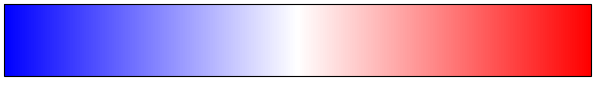
\includegraphics[width=\linewidth,height=0.15in,keepaspectratio]{../bin/colormaps/resource/matplotlib_bwr.png}}};
    %
    \node(apbslabel) [above, inner sep=6pt] at (spectrumbar.north) {30 kT/e};
    \node(apbslabel) [below, inner sep=6pt] at (spectrumbar.south) {-30 kT/e};       
    %
    %
    %
    \node(tetramer)[inner sep=0pt,right=2cm of spectrumbar.east]{\includegraphics[width=\linewidth,height=1.25in,keepaspectratio]{../results/cavity/output/tetramer_cavity_apbs_side_no_ramp_cropped.png}};
    %
    \node(captionB)[inner sep=0pt,above left] at (tetramer.north west) {\normalsize\textbf{\figurepanelb}};
    %
    \path (tetramer.north)++(-0.5,-0.95) coordinate (tetramerROISW1);            
    \path (tetramer.north)++(0.5,-1.8) coordinate (tetramerROINE1);
    \node(tetramerROIrect) [fit={(tetramerROISW1) (tetramerROINE1)}, dashedrectanglefit] {};
    %
    %
    \path (tetramer.west)++(-0.25,0.5) coordinate (chainA_tetramer);           
    \path (tetramer.north)++(-1.5,0) coordinate (chainB_tetramer);
    \path (tetramer.north)++(1.5,0) coordinate (chainAprime_tetramer);
    \path (tetramer.east)++(0.25,0.5) coordinate (chainBprime_tetramer);
    %
    \node(chainAlabel) [above, inner sep=2pt, align=center] at (chainA_tetramer) {Chain A};
    \node(chainBlabel) [above, inner sep=2pt, align=center] at (chainB_tetramer) {Chain B};
    \node(chainAprimelabel) [above, inner sep=2pt, align=center] at (chainAprime_tetramer) {Chain A'};
    \node(chainBprimelabel) [above, inner sep=2pt, align=center] at (chainBprime_tetramer) {Chain B'};
    %
    \node(D144_E174_closeup)[inner sep=0pt,below=1cm of tetramer.south,anchor=north]{\includegraphics[width=\linewidth,height=1.5in,keepaspectratio]{../results/cavity/output/tetramer_cavity_D144_E174_closeup_no_ramp_cropped.png}};
    %
    \node(closeuprectD144E174) [fit=(D144_E174_closeup), dashedrectanglefit] {};
    %
    \path[dashed edge] (tetramerROIrect.south) edge (closeuprectD144E174.north);
    %
    \path (D144_E174_closeup.south west)++(0.5,-0.65) coordinate (cE174label);
    \path (D144_E174_closeup.west)++(1.125,-0.65) coordinate (cE174);
    \node(E174) [above, inner sep=3pt, font=\small, font=\bfseries] at (cE174label) {E174};
    \path[-,thick] (E174.north) edge (cE174.south);
    %
    \path (D144_E174_closeup.south east)++(-0.5,-0.65) coordinate (cD144label);
    \path (D144_E174_closeup.east)++(-1.125,-0.3) coordinate (cD144);
    \node(D144) [above, inner sep=3pt, font=\small, font=\bfseries] at (cD144label) {D144};
    \path[-,thick] (D144.north) edge (cD144.south);
    %
    \node(filament)[inner sep=0pt,below=4.5cm of axialdimer.west,anchor=west]{\includegraphics[width=\linewidth,height=1.25in,keepaspectratio]{../results/cavity/output/filament_cavity_and_yb_blend_cutaway_cropped.png}};
    %
    \node(captionC)[inner sep=0pt,above left] at (filament.north west) {\normalsize\textbf{\figurepanelc}};
    %
\end{tikzcanvas}
\end{conditionalpanel}
\begin{conditionalcaption}
\caption[The electronegative lumen within the cardiac calsequestrin filament]{\textbf{\headingsubsectionsix}. \figurepanelcaptiona Left panel: the interior cavity of the dimer viewed down its long axis. Residues that interact with Yb atoms within the intra-dimer cleft (\maintextfigure~\ref{fig:intra_dimer_interface}) are shown as sticks. All other residues are rendered as surface. Right side: APBS-generated electrostatic surface of the same region. \figurepanelcaptionb The lumen is continuous down the length of filament because of the large solvent cavity formed at each dimer-dimer interface. The APBS-generated electrostatic surface of the lumen (as traced by HOLLOW using a 1.4 \AA\ probe) is shown, with closeup of residues D144 and E174 deep within the electronegative cavity. \figurepanelcaptionc View of the filament and its continuous interior cavity, with Yb sites shown as magenta spheres.}
\label{fig:filament_cavity}
\end{conditionalcaption}
\end{figure}